\let\negmedspace\undefined
\let\negthickspace\undefined
\documentclass[journal,12pt,twocolumn]{IEEEtran}

 \usepackage{gensymb}

 \usepackage{polynom}

\usepackage{amssymb}

\usepackage[cmex10]{amsmath}
\usepackage{amsthm}
\usepackage{graphicx}

 \usepackage{stfloats}

 \usepackage{bm}
\usepackage{longtable}

\usepackage{enumitem}
 

\DeclareMathOperator*{\Res}{Res}
\DeclareMathOperator*{\equals}{=}


\begin{document}

\bibliographystyle{IEEEtran}


\providecommand{\brak}[1]{\ensuremath{\left(#1\right)}}


\providecommand{\system}{\overset{\mathcal{H}}{ \longleftrightarrow}}
\newcommand{\question}{\noindent \textbf{Question: }}	
\newcommand{\solution}{\noindent \textbf{Solution: }}

\providecommand{\dec}[2]{\ensuremath{\overset{#1}{\underset{#2}{\gtrless}}}}



\vspace{3cm}
\title{I.C.S.E 10, 2018}

\author{ Burra Vishal Mathews\\CS21BTECH11010}
	


\maketitle
\question : 3(a) : 
 If $(x+2)$ and $(x+3)$ are factors of $x^3+ax+b$, find the values of $'a'$ and $'b'$.\\


\solution
    According to the question :

    $x+2$ and $x+3$ are factors of $x^3+ax+b$.\\
    Then, -2 and -3 are solutions of the equation \\
    \begin{equation}
    \label{maineq}
        x^3+ax+b=0
    \end{equation}
    On substituting $x=-2$  int the equation (\ref{maineq})
    \begin{align*}
        \implies \brak{-2}^3+a\brak{-2}+b&=0\\ 
        \implies 2a-b&=-8
    \end{align*}
    The value of $b$ in terms of $a$ is :
    \begin{equation}
    \label{eq1}
        b=2a+8
    \end{equation}
    \\
    On substituting $x=-3$ in the equation (\ref{maineq})$$\implies \brak{-3}^3+a\brak{-3}+b=0$$
    \begin{equation}
    \label{eq2}
        \implies 3a-b=-27
    \end{equation}
    On substituting equation (\ref{eq1}) in equation (\ref{eq2})
    \begin{align*}
        \implies 3a-\brak{2a+8}&=-27\\
        \implies a-8&=-27\\
        \implies a&=-19
    \end{align*}
    Substitute value of $a$ in equation (\ref{eq1}) 
    \begin{align*}
    \implies b&=2\brak{-19}+8\\
    \implies b&=-30\\
    \end{align*}
    $ \therefore $ The value of $a = -19$ and value of $b = -30$.\\
    
    Using values of $a$ and $b$, equation (\ref{maineq}) can be re-written as :
    \begin{equation}
    \label{Peq}
        x^3-19x-30=0
    \end{equation}
    This can be verified by plotting the graph of the equation
    \begin{equation}
    \label{grapheq}
        y=x^3-19x-30
    \end{equation}
\begin{figure}[h]
    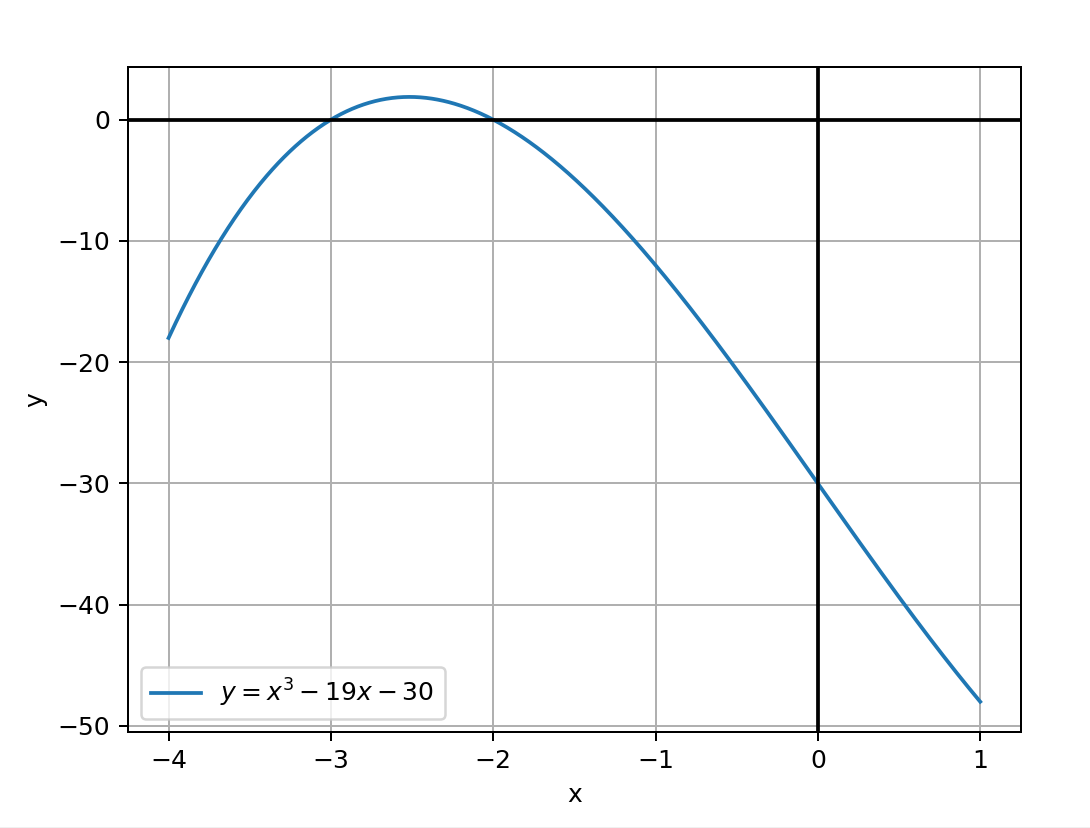
\includegraphics[width=0.5\textwidth]{Graph.png}
    \caption{Graph of equation (\ref{grapheq}) intersects X-axis at $x=-3$ and $x=-2$ }
    \label{graph}

\end{figure}



\end{document}